\chapter{智能体意图调度理论和方法}
本章主要介绍本文提出的相关方法所依赖的核心算法--蒙特卡洛树搜索算法以及其在目标计划树模型下的具体应用。
\section{蒙特卡洛方法}
蒙特卡洛方法是一类基于随机采样对决策或状态进行评估的方法。
% 重要性
该方法在多个领域都有重要应用,例如在棋类游戏中进行随机模拟采样,以此来对不同决策所带来的收益进行评估;又如在统计物理学与数学问题渗透问题中,利用现代计算机的高速计算能力进行随机采样以计算不同情况下的渗透概率。
% 特点,举例说明,model probability,额外说明episodic
蒙特卡洛方法的特点在于使用多次随机采样结果的平均值对某一状态或决策进行价值评估。其样本来源可以是智能体与实际环境的交互流程,也可以是智能体基于对环境的认知,进行的随机模拟。例如,在棋类游戏中,若需对当前棋手的胜率进行估计,则可以基于当前棋局进行多次随机模拟,每次模拟都在某一方获胜的情况下停止。最终统计各棋手在所有模拟流程中的胜利与失败次数,并基于此计算胜率。虽然蒙特卡洛方法需要环境模型,例如棋类游戏的规则,但是其并不需要精确的决策结果的概率分布,例如对手棋手的策略,而仅需要可以生成样本的模型。在众多领域,获得模型的生成样本比获得完全的概率分布更加容易。另有一点需要注意的是,蒙特卡洛方法仅应用于幕式模型(Episodic Model),即环境的运行最终会停止,而不会无限运行下去。

% 优点
蒙特卡洛方法有多个优点,
首先,它是一个领域无关(Domain Independent)的方法,也就是说它仅需知道环境的基本运行规则,而不需要环境的所有信息。
%
其次,蒙特卡洛方法可以基于多次的随机采样采样提供较为准确的价值评估,基于大数定律(Law Of Large Numbers),随机变量的期望值可以由很多个样本值的平均值近似求得,因此其准确性在理论上得到保障。
%
另外,在随机性较强、可能性众多的场景,蒙特卡洛方法由于其自身随机性的特点,在进行采样时会考虑到所有可能的情况,而不会只考虑到其中一部分。
%
最后,蒙特卡洛方法可仅针对于环境的某一个状态进行评估,而不需掌握环境所有可能状态的评估值,因此当需要对环境的某一特定状态进行价值评估,蒙特卡洛方法比其他方法(如动态规划方法)更加高效。

% 缺点
然而,蒙特卡洛方法也有一些缺点。例如基于其随机采样得到的评估值仅仅只是近似值,而不是一个准确值。在一些特定场景下,考虑到计算开销,蒙特卡洛方法只能进行少量的随机采样,而无法进行多次的随机采样,这种情况下即使有大数定律的支撑,由于样本量少,使得评估价值与实际值会有较大偏差。
%
另外,蒙特卡洛方法对多个不同环境状态的评估都是相互独立的,这意味着对某一个环境状态的评估过程以及结果并不会影响其他环境状态的评估。这种特性使得人们无法通过蒙特卡洛方法建立不同环境状态直接的联系。相较于此,树搜索则可以基于不同环境状态之间的因果关系以及动作结果的概率分布,构建树形结构,其清晰直观地展现了不同环境状态直接的关联性。树形结构明确地展现了不同动作所导致的结果以及一连串动作导致的结果等,这在众多决策问题中可以提供有效的指导性。而蒙特卡洛方法仅仅只有基于随机采样得到的数值。
\section{蒙特卡洛树搜索(Monte-Carlo Tree Search)}
蒙特卡洛树搜索是一种针对决策问题的启发式搜索算法\cite{DBLP:conf/aiide/ChaslotBSS08,chaslot2006monte,DBLP:conf/ecml/KocsisS06},其结合了蒙特卡洛方法随机性的优点以及树搜索精确性的优点,在人工智能领域有着重要应用。2016年,研究人员将蒙特卡洛树搜索与神经网络(Neural Network)相结合,开发出了能够击败世界围棋冠军的ALphaGo\cite{DBLP:journals/nature/SilverHMGSDSAPL16},引起各界广泛关注。此外,蒙特卡洛树搜索还被应用在其他游戏中,如桥牌、克里比奇牌以及电子游戏《全面战争:罗马2》中。最初蒙特卡洛树搜索主要应用于游戏领域,但其树搜索以及随机模拟的特性使得它可被应用于其他问题领域,只需问题的求解过程可以通过树形结构表示即可。

蒙特卡洛树搜索通常在智能体当前的环境状态下运行,用于求解当前状态的最佳决策。在执行完一个决策之后,智能体进入到下一个环境状态,这时蒙特卡洛树搜索将被再次调用用于求解下次的决策,如此循环往复直到智能体到达某个最终状态。每一次蒙特卡洛树搜索的执行都是基于当前环境状态的对将来执行过程的模拟。

% core idea
蒙特卡洛树搜索的核心思想在于在有限给定的计算资源下专注于对收益最大或者最有潜力的模拟执行路径进行分析,以得到最优决策。基于当前的环境状态,其使用模拟执行轨迹的评估值对初始部分的执行轨迹进行评估,并基于评估值对初始执行轨迹进行拓展,被拓展的部分为收益最大或者最有潜力的决策。由此,初始部分的执行轨迹随着蒙特卡洛树搜索的执行越来越具体,并随着扩展,初始部分的执行轨迹占比也越来越大。
%rollout
在每一次的模拟执行过程中,随机模拟执行的流程占比最大。随机模拟执行的评估值最终将用于刻画初始决策的价值(这些决策往往是智能体在不久的将来所可能作出的决策)。在随机模拟过程中,智能体将执行随机策略(Rollout Policy),只要随机策略相对简单且环境模型并不复杂,蒙特卡洛树搜索可以在有限的计算资源下生成大量模拟执行路径。
% only part of state-action paris are considered
模拟执行的流程只与一部分初始决策有相关性,这些初始决策与其所处的环境状态共同构成了树形结构。其中每个节点记录了环境状态,该状态被经历的次数以及状态的评估值。每个边对应于智能体的一个决策。蒙特卡洛树搜索增量式地基于模拟路径的评估值对树进行扩展,被拓展的部分为价值高或者有潜力的状态。每一次的模拟执行都是从根节点(对应于智能体的当前状态)出发,进过部分子节点并最终达到某个叶子结点后离开搜索树;离开搜索树之后,根据随机策略进行多次的随机模拟得到评估值用于对经历过的树节点进行价值更新。

%
在树中进行搜索时,基于每个节点的价值进行选择性的搜索,树中的搜索策略被称为树策略(Tree Policy)。树策略可以用于平衡探索(Exploration)与开发(Exploitation),即在探索最有潜力的决策与开发最有价值的决策间进行权衡。其中最有潜力的决策为在模拟时经历次数少的决策,而最有价值的决策对应于导致最终随机模拟结果的评估值高的决策。
% UCB
在蒙特卡洛树搜索中,树策略一般使用UCB(Upper Confidence Bound,UCB)\cite{DBLP:journals/ml/AuerCF02}规则:

\begin{equation}
UCB = \overline{X}_{a} + c\sqrt{\frac{2\ln N}{N_a}}
\end{equation}

其中,$\overline{X}_{a}$为决策$a$价值的平均值,$N_a$为决策$a$被执行的次数,$N$为执行的总次数,$c$为某个大于0的常数,其作用为控制探索的程度($c$越大,该算法越倾向于探索)。

% specific
蒙特卡洛树搜索具体包括四个阶段:选择(Selection),扩展(Expansion),模拟(Simulation)以及回溯(Back-Propogation)。图\ref{fig:mcts_process}中展示了运行一次蒙特卡洛树搜索的过程。

\begin{figure*}[htb]
\centering
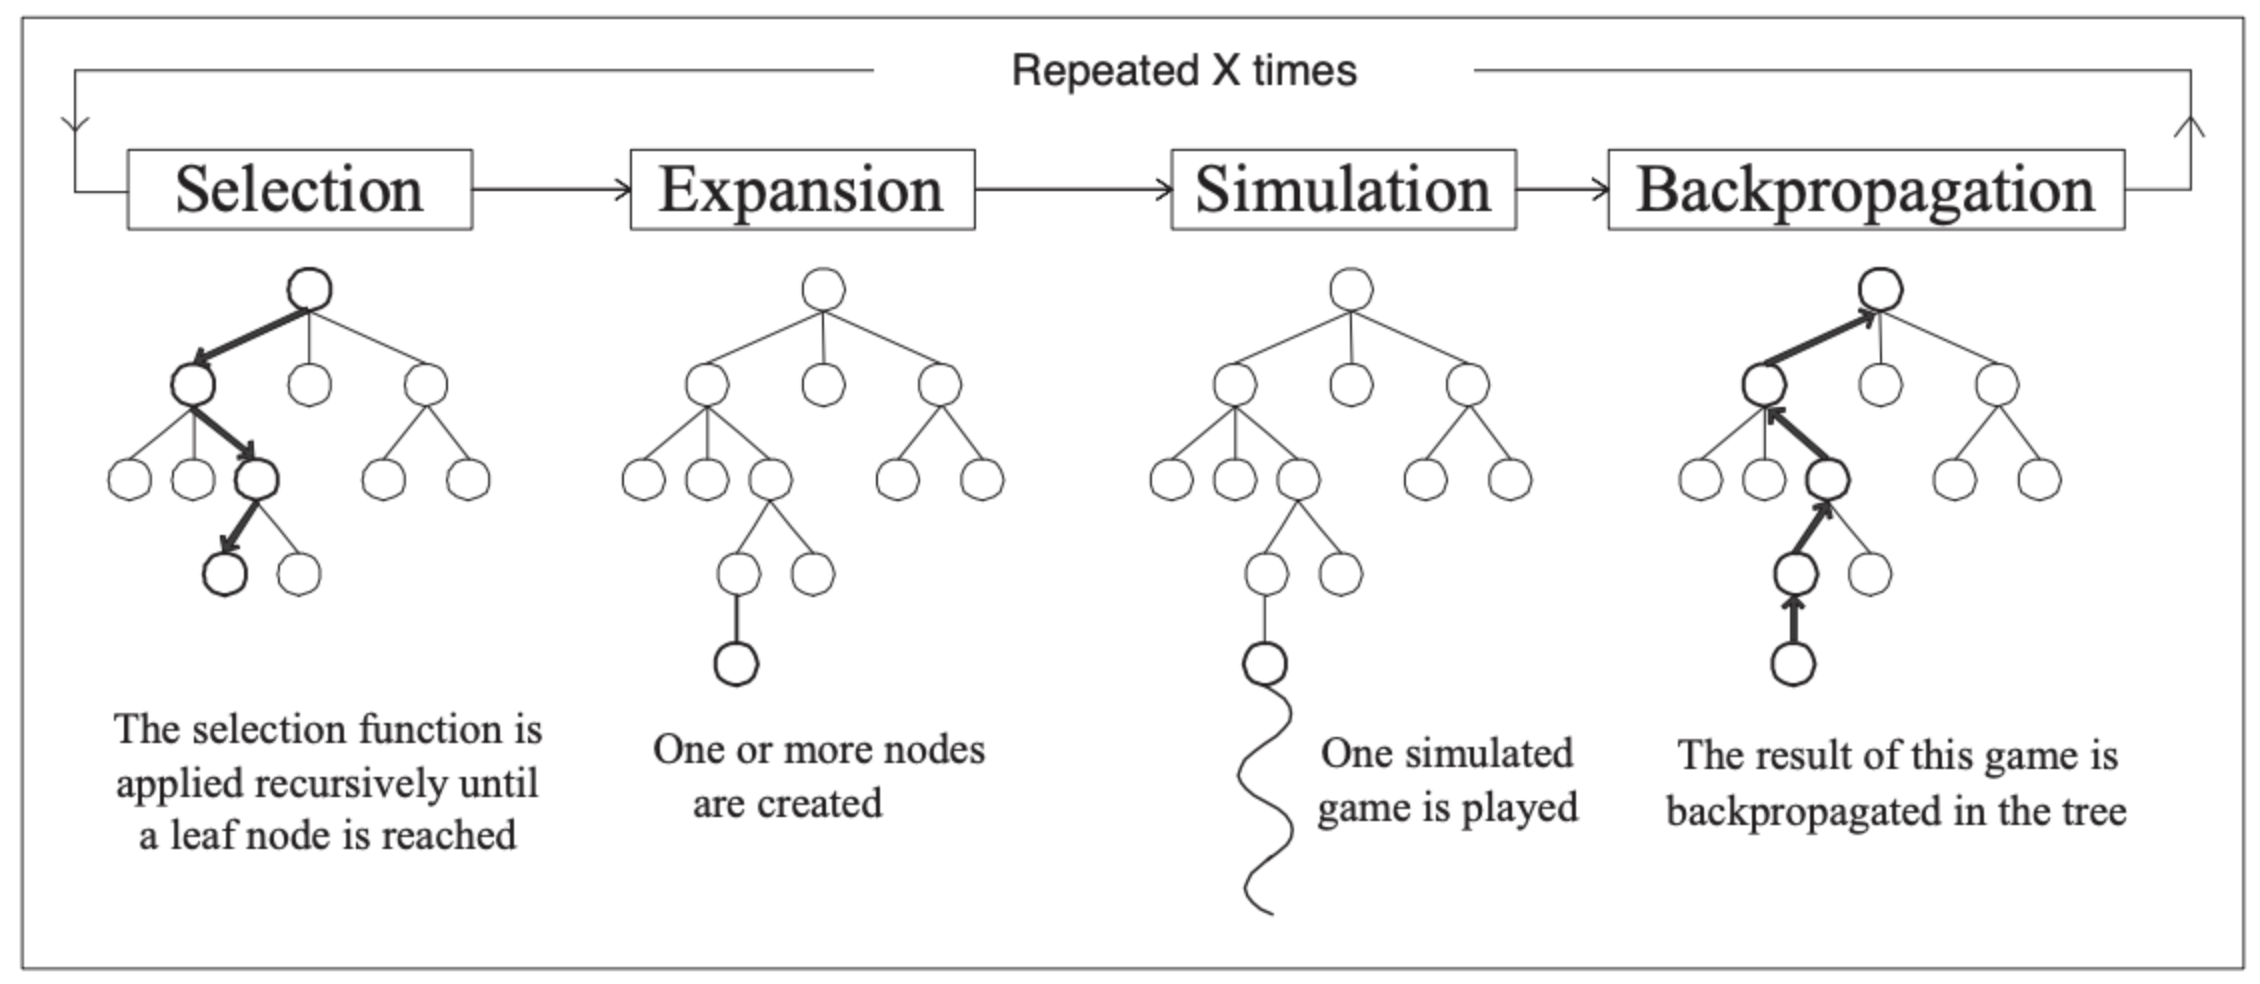
\includegraphics[width=0.9\textwidth]{./figs/mcts_process}
\bicaption{MCTS流程\cite{Sutton2005ReinforcementLA}}{Outline of MCTS\cite{Sutton2005ReinforcementLA}}
\label{fig:mcts_process}
\end{figure*}

\paragraph{选择}
在选择阶段,自根节点开始,根据树策略不断迭代选择子节点,直到到达某个叶子结点$n_e$。最终选中的叶子结点将用于接下来的扩展。
\paragraph{扩展}
在扩展阶段,基于被选中的叶子结点$n_e$,生成一个或多个新节点作为$n_e$的子节点。这些新生成的节点根据$n_e$节点中的状态所能执行的动作而生成。每一个新节点都对应于在$n_e$状态下执行一个动作的结果,而连接$n_e$与新节点的边则对应于该动作的执行。需要注意的是,若$n_e$状态下无可执行的动作,则不会有新的节点生成。新生成的节点用于下一步的模拟。
\paragraph{模拟}
在模拟阶段,首先选中某一个新生成的节点$n_s$(如果在扩展阶段没有新节点的生成,则选择当前叶子结点),从$n_s$节点中的状态开始,使用某个随机策略进行随机模拟执行,直至某个最终状态。至此可知,蒙特卡洛树搜索的一次完整的模拟执行轨迹由两部分组成:在树搜索阶段根据树策略生成的执行轨迹,以及在随机模拟阶段根据随机策略生成的执行轨迹。随机模拟过程中使用的策略可以是完全随机,以应用于多种问题场景,也可以根据具体的问题场景由用户自行控制以获得更准确的价值评估或节省计算开销。
\paragraph{回溯}
最后,在回溯阶段,上一阶段获得的最终评估值被反向传播至搜索树中所经历的每个节点以更新其相应的价值。

蒙特卡洛树搜索循环迭代地执行上述四个步骤直到用尽给定的时间或耗尽其它的计算开销。最终,根据某种策略,根节点状态下的某个动作被选中并返回给智能体作为最终的决策。最终的选择策略有多种,例如选择根节点状态下可执行的价值最高的动作,或者是选择被访问次数最多的动作等。用户可以根据具体的应用场景自行选择合适的策略。总之,该最终选择的动作即为智能体下一步真实执行的动作。
%
在执行完该选中的动作之后,环境被改变,进入下一个状态,蒙特卡洛树搜索再次被执行以确定下一个要执行的动作。新一轮的算法执行可以根据新的环境状态重新自根节点开始构建搜索树,也可以基于上一次算法执行所生成的搜索树进行构建,以节省计算开销。

% @TODO: advantages of MCTS

\section{目标计划树模型下MCTS的应用}\label{SA}
Yao等人提出基于蒙特卡洛树搜索的\SA \cite{DBLP:conf/atal/YaoL16}算法用于在目标计划树模型下对智能体的意图进行调度。本节的主要内容是对\SA 算法进行介绍(由于\SA 算法的应用场景与本文有所不同,所以略去了算法的一些无关部分)。

\SA 算法有4个输入参数:
\begin{enumerate}
  \item 智能体当前的意图集合 I(以目标计划树的形式表示),
  \item 智能体当前所处的环境状态 E,
  \item 每次算法所执行的迭代次数 $\alpha$, 
  \item 以及每次迭代迭代中随机模拟的执行次数 $\beta$,
\end{enumerate}
其中$\alpha$和$\beta$参数决定了算法运行的计算开销,可由用户自定义。\SA 最终返回某个意图中的下一步选择以供智能体在当前周期执行。\SA 算法的具体流程如算法\ref{alg:SA}所示:

\begin{algorithm}
\caption{返回当前周期执行的动作}\label{alg:SA}
  \begin{algorithmic}[1]
    % \PROCEDURE{$SA(I, E,\alpha,\beta)$}{}
    \STATE input:$(I, E,\alpha,\beta)$
    \STATE $n_0 \gets node_0(I,E)$ \label{root}
    \FOR{$i \gets 1,\alpha$} \label{iteration begin}
      \STATE $n_e \gets MAX-UCT-LEAF-NODE(n_0)$ \label{selection}
      \STATE $EXPAND(n_e)$ \label{expansion}
      \STATE $n_s \gets RANDOM-CHILD(children(n_e))$ \label{simulation begin}
      \STATE $S \gets \emptyset$
      \FOR{$j \gets 1, \beta$}
        \STATE $S \gets S \cup SIMULATE(n_s)$
      \ENDFOR \label{simulation end}
      % @TODO: max or average?
      \STATE $V_{best} \gets maxValue(S)$
      \STATE $BACKUP(n_s, V_{best})$ \label{back}
      \ENDFOR \label{iteration end}
      \STATE \RETURN $BEST-NEXT-STEP(n_0, f_b)$
    % \ENDPROCEDURE
  \end{algorithmic}
\end{algorithm}

其中$I=\{(t_1,s_1), \dots, (t_n, s_n)\}$,$t_i$表示第$i$个目标计划树(即第$i$个意图),$s_i$表示底$i$个目标计划树的当前步骤。算法流程从代表智能体当前所处状态与意图的根节点(第\ref{root}行)开始,迭代地进行模拟执行并扩展搜索树。算法的主体循环部分(第\ref{iteration begin}-\ref{iteration end}行)对应于蒙特卡洛树搜索的四个阶段:选择、扩展、模拟以及回溯。
% selection
第\ref{selection}行对应了选择阶段:从根节点$n_0$开始,根据基于UCB的树策略不断进行选择,直到某个叶子结点$n_e$。
% expansion
第\ref{expansion}行对应了扩展阶段:基于智能体在$n_e$状态下可以进展的意图,生成新的树节点。在这一阶段,依次对智能体的每个目标计划树进行检查,若目标计划树当前的步骤为动作节点,那么直接生成一个新的搜索树节点,对应于执行该动作的结果;若当前步骤为(子)目标,那么检查是否有可用的计划,若有可用计划则递归地对每个可用计划的第一个步骤进行检查:若为动作节点则直接生成相应的新搜索树节点,否则继续检查。由此得知,每一个新节点就是一条意图的部分执行路径,且该路径的最后一个执行步骤为动作。最后,随机选中一个生成的节点$n_s$作为接下来模拟阶段的开始状态。
% simulation
第\ref{simulation begin}-\ref{simulation end}行对应了模拟阶段:在该阶段,基于完全随机的策略(或者用户指定策略)进行目标计划树的进展,直到无法执行下去或所有目标都被实现,即所有当前步骤的前置条件都不满足(对于目标则是无可用计划),或所有顶层目标指定的状态都被实现。
% backup
在$\beta$次的模拟流程结束之后,选择$\beta$次模拟中最大的评估值进行反向传播。该价值反向传播至从$n_s$到根节点$n_0$路径上的所有节点。除了智能体的意图以及环境状态信息,每个节点还记录了其他统计信息:节点被访问次数,回溯价值总和以及最佳的回溯价值。

在$\alpha$次的循环执行之后,\SA 算法最终基于某个评价标准$f_b$返回当前周期(对应于树搜索的根节点$n_0$)最佳的意图进展策略(第\ref{back}行)。$BEST-NEXT-STEP$方法根据$f_b$对根节点的孩子节点进行比较,并返回到达某个最优节点$n_p$的边(即下一步的选择和执行的动作)。$f_b$可以由用户自定义,如以节点的访问次数为标准或以节点的最高价值为标准等。最终智能体将实际执行该选择的步骤,并在执行之后根据环境反馈更新自身信念和意图。

\subsection{\SA 算法与BDI智能体的实践推理过程}
第\ref{background}章中提到BDI智能体的实践推理过程包括慎思与手段推理,分别对应于意图选择和计划选择。然而,在\SA 算法中,慎思与手段推理实际上被合并为一步。另外,\SA 算法针对的问题是如何去实现给定的一组目标,而对于要实现哪些目标则在\SA 算法的考虑范围之外,通常由用户给定。当智能体接收到一个新目标之后,\SA 算法不仅要确定接下来要实现哪个目标,还要确定使用哪一个计划来实现该目标;在该过程中还要考虑到多个意图之间的相互交错带来的影响,避免负面的影响并利用多意图间的协同效应,最终得到收益最大的意图进展路径。

%
在众多智能体编程语言中,意图选择和计划选择策略往往是默认的先来先服务(First In First Out,FIFO)或轮询(Round Robin,RR)算法,或需要用户自定义,例如在Jason\cite{bordini2007programming}中,计划选择时默认选择可用的第一个计划,而意图选择算法为轮询。
%
另外Jason也提供用户自定义的策略编程接口$S_O$和$S_I$分别对应于计划选择策略和意图选择策略。
% compare to jason
虽然提供自定义决策编程接口可以使得智能体更加灵活,但是自定义策略需要有一定程度的某个问题领域的专业知识。若要将其应用多种场景,则需要进行多次的策略定制。另外,决策策略一般为智能体编程语言层面的设计,使用不同智能体编程语言对决策策略的自定义方式可能不尽相同,这一定程度上增加了程序员的负担。对比之下,\SA 算法则可以让用户专注于需要解决的问题本身,即如何定义价值函数,而无需考虑编程语言的底层实现。

%
在目标计划树中,每个节点都有其相关的条件:目标有其目标条件,计划有其前置条件,动作有其后置条件。虽然这些条件由用户自行设定,需要一定的额外工作,但是于\SA 算法可以有效利用这些条件来避免意图间的冲突以及利用意图间的协同效应以高效地执行智能体程序。
